\chapter{Learned policies}\label{app:Policies}

In Chapter \ref{sec:RL-Solution_methods}, we mentioned that 'solving' in a \ac{RL} context means finding an optimal policy. An optimal policy assigns an action to every state. However, our learning experiments did not lead to a (converged) policy for the entire state-space. We were only interested in finding (sub-)optimal trajectories towards the goal. This is true for most \ac{RL} experiments. Convergence to a solution in the entire state-space is almost never possible for model-free or model-learning methods as parts of the state-space will never or only rarely be visited by the system. In practice however, it is often not needed to converge to a solution in the entire state-space as we only need a control policy along interesting trajectories (towards the goal).

In this Appendix we show the final polices of the different algorithms that we have used in our research.


\section{Converged policy}
In order to get insight in how the optimal policy looks, we executed a (random) Dyna experiment using the exact model. We executed 10000 trials and used the exact model to generate $N_m=10$ state-transitions per time step. These settings should lead to a converged solution throughout the entire state-space.

\figref{fig:PS-converged_policy} shows the resulting policy. Although some minor artifacts are still visible, the obtained policy will be used as (an approximation of) the fully converged optimal policy.



\section{SARSA policy}
The obtained policy using SARSA is shown in \figref{fig:PS-SARSA_policy}. The learning results showed that the reward per trial converged to a final value. The policy however, has not converged in the entire state-space. The regions that show a converged policy, are the parts that were visited frequently by the system.

\begin{figure}[htbp]
\centering
\subfigure{
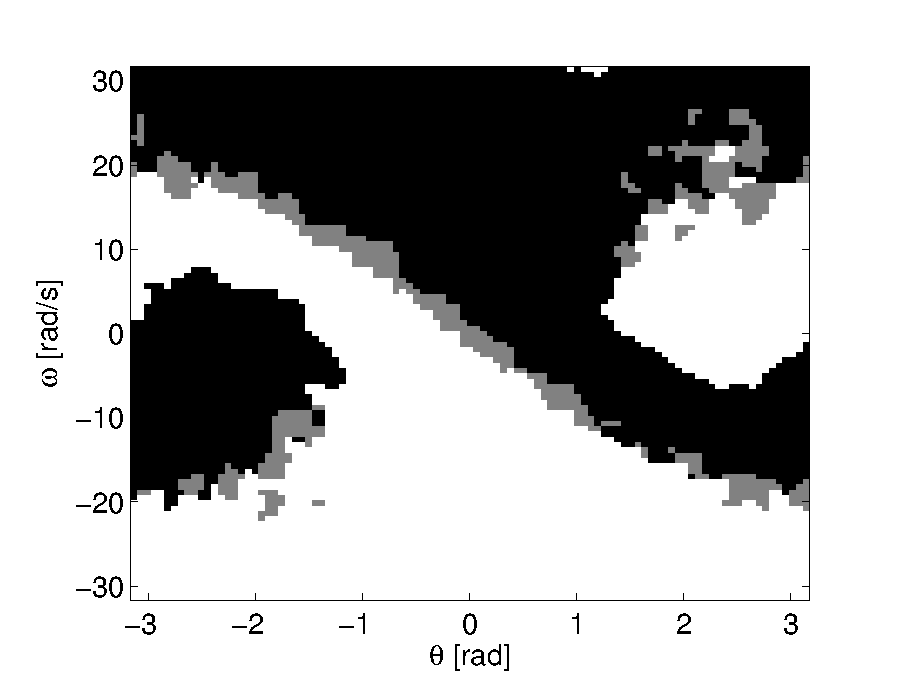
\includegraphics[width=.4\textwidth]{Figures/PS-invpend_optimalpolicy}
\label{fig:PS-converged_policy}
}
\subfigure{
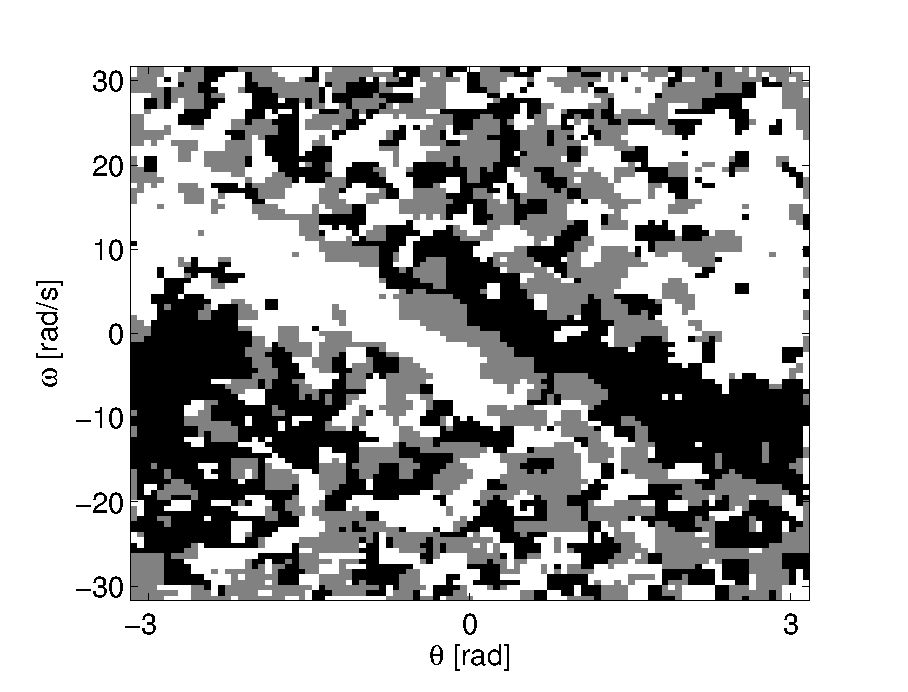
\includegraphics[width=.4\textwidth]{Figures/PS-SARSA_policy}
\label{fig:PS-SARSA_policy}
} 
\caption[Final policy using SARSA]{Comparison of the optimal policy to the obtained policy using SARSA. \subref{fig:PS-converged_policy} shows the optimal policy obtained using Dyna and the exact model, \subref{fig:PS-SARSA_policy} shows the final SARSA policy. The white, gray and black areas correspond to control voltages of +3V, 0 and -3V respectively.}
\label{fig:PS-SARSA_policies}
\end{figure}


\newpage
\section{Dyna policies}
The obtained policies using Dyna are shown in \figref{fig:PS-DYNA_policies}. The policies are converged in a larger part of the state-space than the SARSA algorithm. This is due to the randomly selected model-based updates. This leads to learning in a larger part of the state-space than with SARSA.

\begin{figure}[htbp]
\centering
\subfigure[{$[\delta_\theta,\delta_\omega]=[0.001,0.01]$}]{
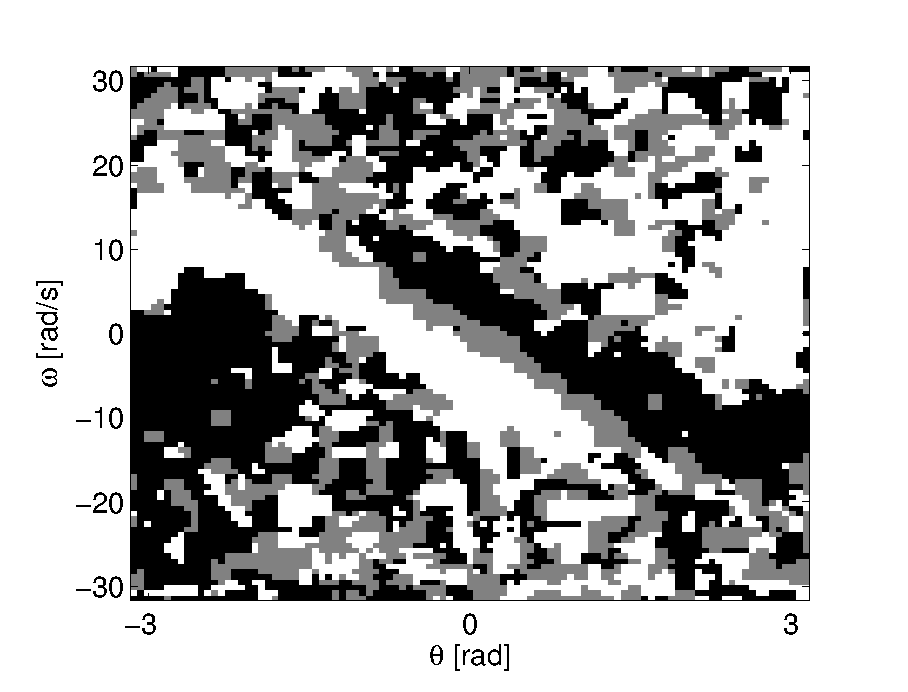
\includegraphics[width=.4\textwidth]{Figures/PS-DYNA1_policy}
\label{fig:PS-DYNA1_policy}
}
\subfigure[{$[\delta_\theta,\delta_\omega]=[0.01,0.1]$}]{
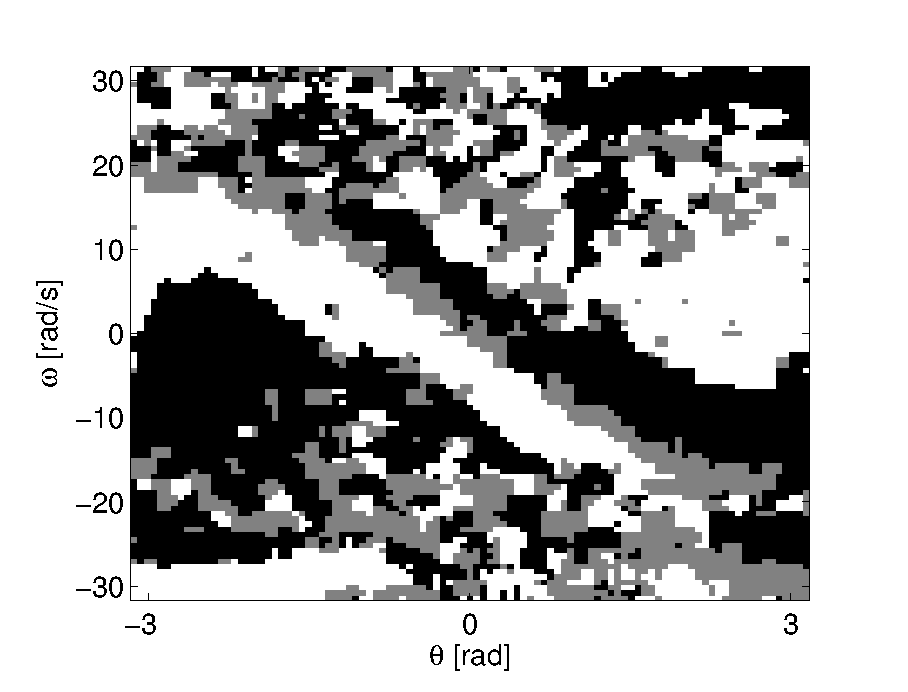
\includegraphics[width=.4\textwidth]{Figures/PS-DYNA2_policy}
\label{fig:PS-DYNA2_policy}
} \\
\subfigure[{$[\delta_\theta,\delta_\omega]=[0.2094,2.0944]$}]{
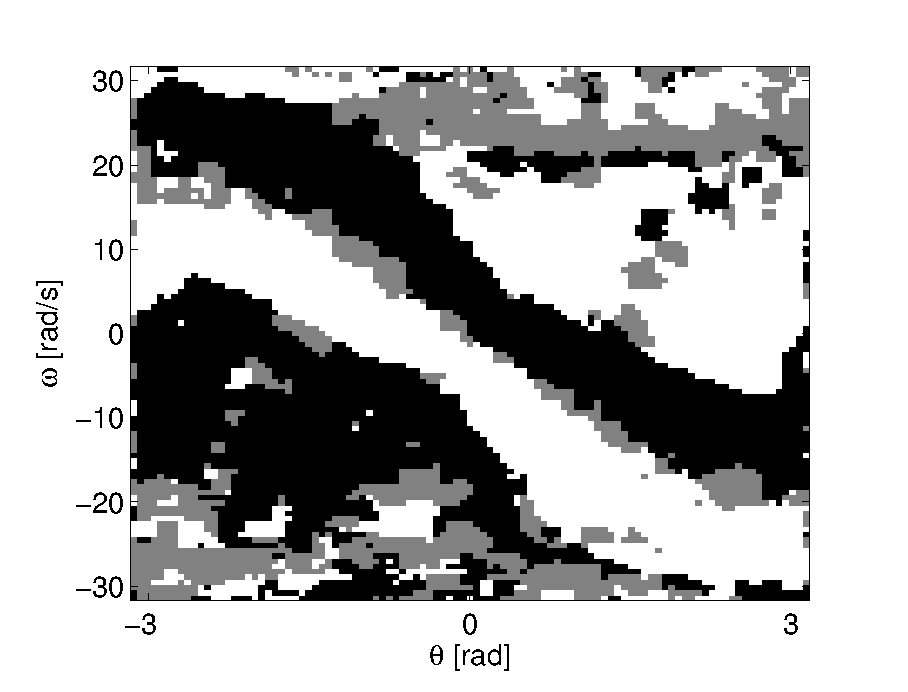
\includegraphics[width=.4\textwidth]{Figures/PS-DYNA3_policy}
\label{fig:PS-DYNA3_policy}
} 
\subfigure[{$[\delta_\theta,\delta_\omega]=[\infty,\infty]$}]{
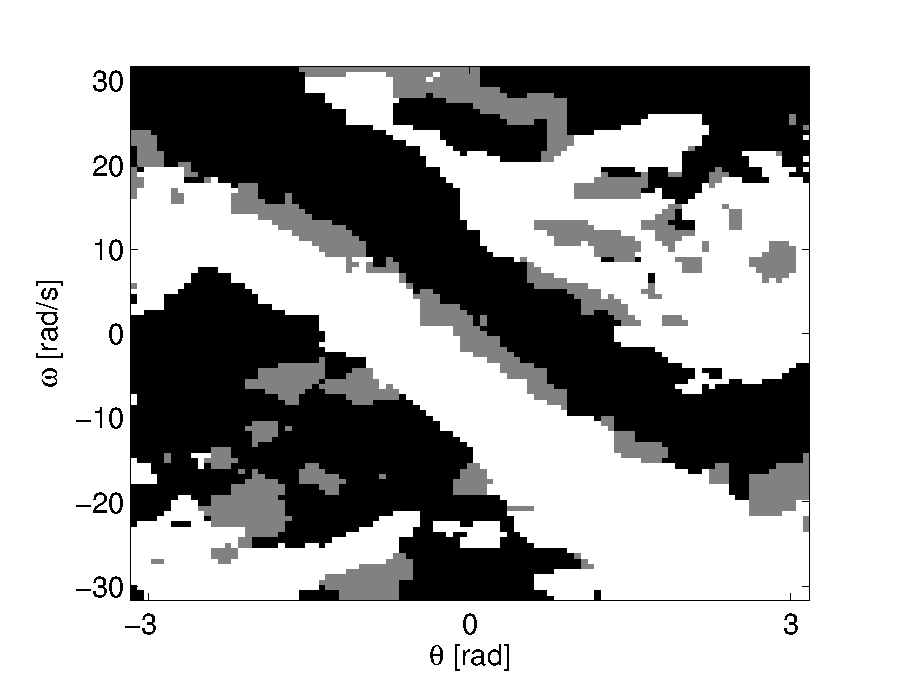
\includegraphics[width=.4\textwidth]{Figures/PS-DYNA4_policy}
\label{fig:PS-DYNA4_policy}
} 
\caption[Final policy using Dyna]{Comparison of the final policies using Dyna. \subref{fig:PS-DYNA1_policy}, \subref{fig:PS-DYNA2_policy}, \subref{fig:PS-DYNA3_policy} and \subref{fig:PS-DYNA4_policy} show the obtained policies using \acs{LLR} with increasing prediction interval limits. The white, gray and black areas correspond to control voltages of +3V, 0 and -3V respectively.}
\label{fig:PS-DYNA_policies}
\end{figure}


\newpage
\section{Prioritized Sweeping policies}
The obtained policies using \ac{PS} are shown in \figref{fig:PS-PS_policies}. Although \ac{PS} resulted in faster learning than Dyna, the resulting policies look worse than in the Dyna setting. This indicates that the resulting trajectory towards the goal may be found fast, but this does not mean that a policy has been found for the entire state-space.

\begin{figure}[htbp]
\centering
\subfigure[{$[\delta_\theta,\delta_\omega]=[0.001,0.01]$}]{
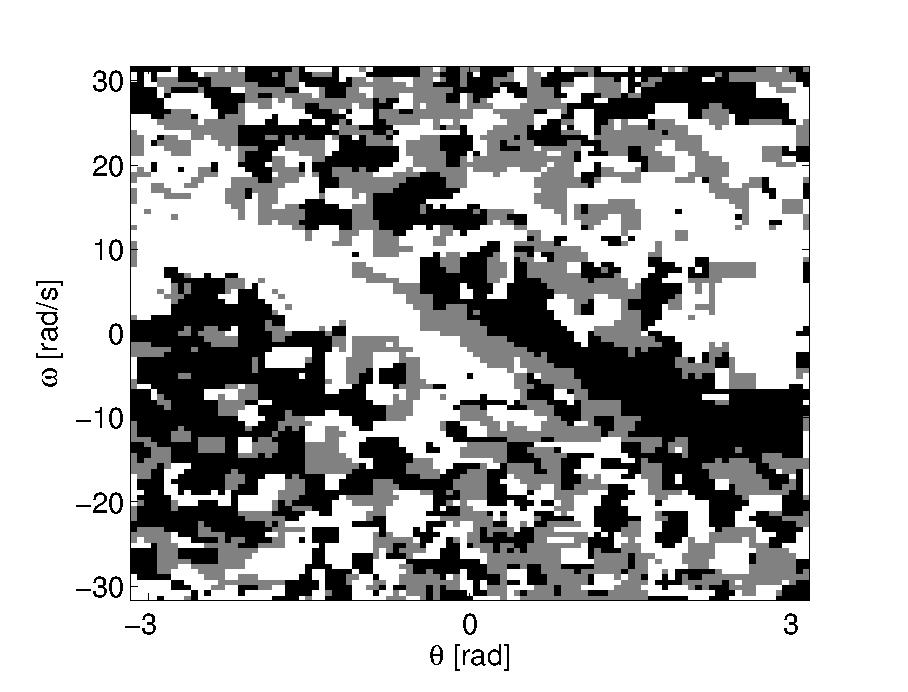
\includegraphics[width=.4\textwidth]{Figures/PS-PS1_policy}
\label{fig:PS-PS1_policy}
}
\subfigure[{$[\delta_\theta,\delta_\omega]=[0.01,0.1]$}]{
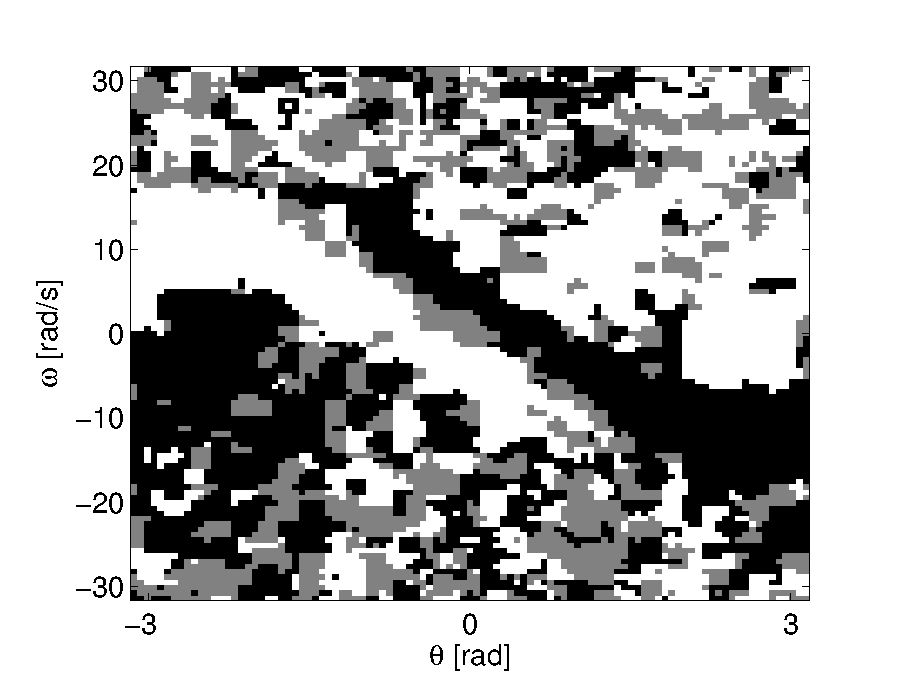
\includegraphics[width=.4\textwidth]{Figures/PS-PS2_policy}
\label{fig:PS-PS2_policy}
} \\
\subfigure[{$[\delta_\theta,\delta_\omega]=[0.2094,2.0944]$}]{
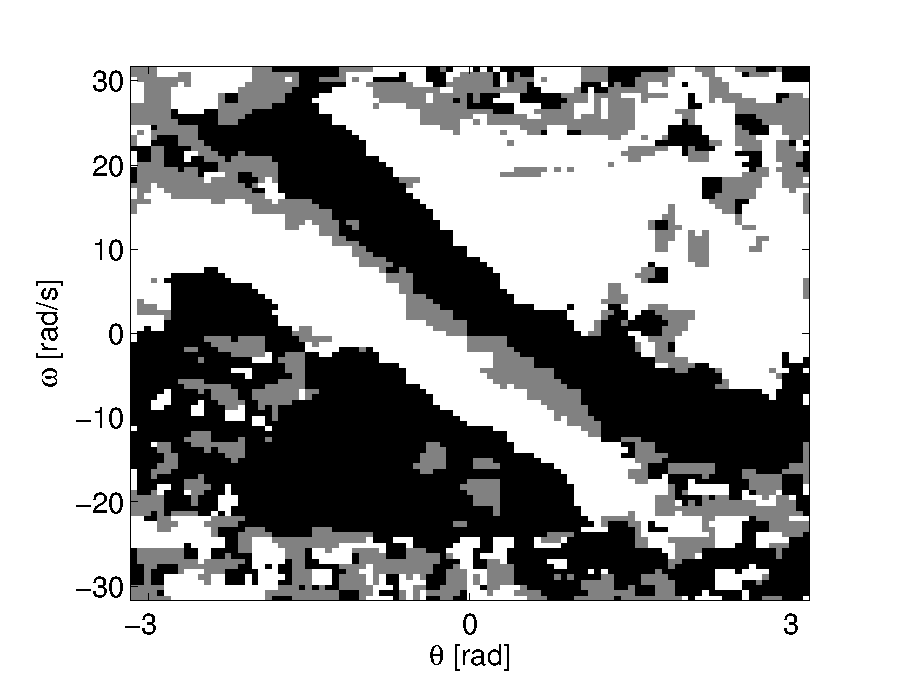
\includegraphics[width=.4\textwidth]{Figures/PS-PS3_policy}
\label{fig:PS-PS3_policy}
} 
\subfigure[{$[\delta_\theta,\delta_\omega]=[\infty,\infty]$}]{
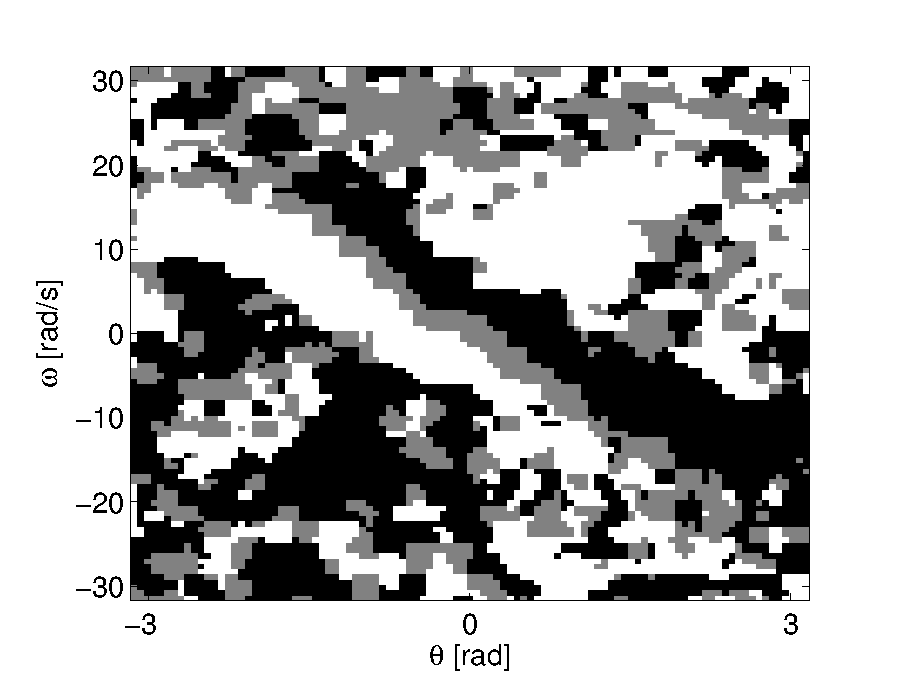
\includegraphics[width=.4\textwidth]{Figures/PS-PS4_policy}
\label{fig:PS-PS4_policy}
} 
\caption[Final policy using \acs{PS}]{Comparison of the final policies using \ac{PS}. \subref{fig:PS-PS1_policy}, \subref{fig:PS-PS2_policy}, \subref{fig:PS-PS3_policy} and \subref{fig:PS-PS4_policy} show the obtained policies using \acs{LLR} with increasing prediction interval limits. The white, gray and black areas correspond to control voltages of +3V, 0 and -3V respectively.}
\label{fig:PS-PS_policies}
\end{figure}


\newpage
\section{Look Ahead Dyna policies}
The obtained policies using \ac{LA Dyna} are shown in \figref{fig:PS-LA_policies}. The policies have about the same quality as the for the \ac{PS} case. Again, faster learning (compared to Dyna) does not result in a better final policy.

\begin{figure}[htbp]
\centering
\subfigure[{$[\delta_\theta,\delta_\omega]=[0.001,0.01]$}]{
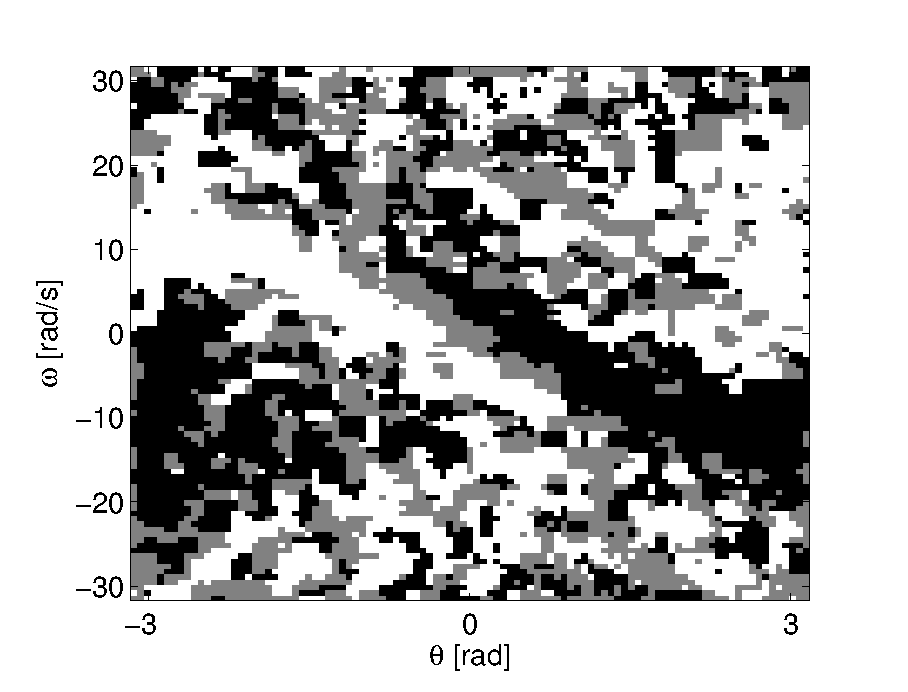
\includegraphics[width=.4\textwidth]{Figures/PS-LA1_hLLR_policy}
\label{fig:PS-LA1_policy}
}
\subfigure[{$[\delta_\theta,\delta_\omega]=[0.01,0.1]$}]{
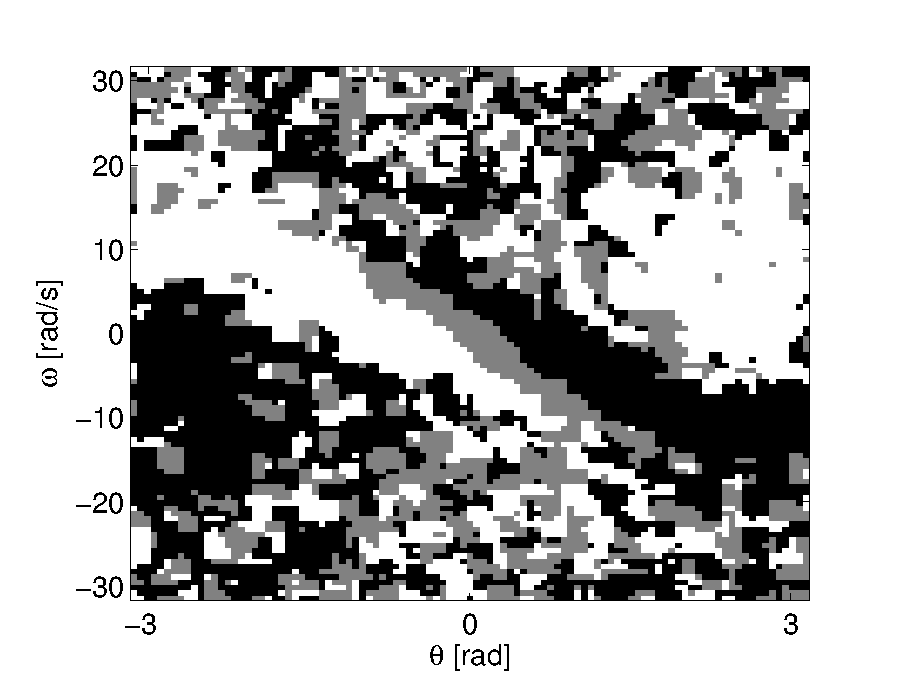
\includegraphics[width=.4\textwidth]{Figures/PS-LA2_policy}
\label{fig:PS-LA2_policy}
} \\
\subfigure[{$[\delta_\theta,\delta_\omega]=[0.2094,2.0944]$}]{
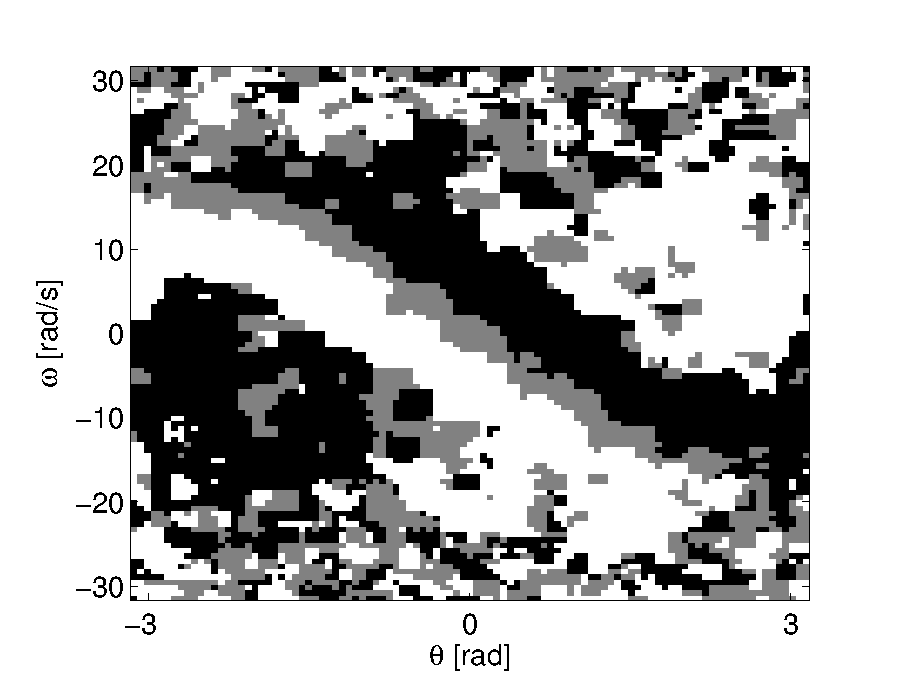
\includegraphics[width=.4\textwidth]{Figures/PS-LA3_policy}
\label{fig:PS-LA3_policy}
} 
\subfigure[{$[\delta_\theta,\delta_\omega]=[\infty,\infty]$}]{
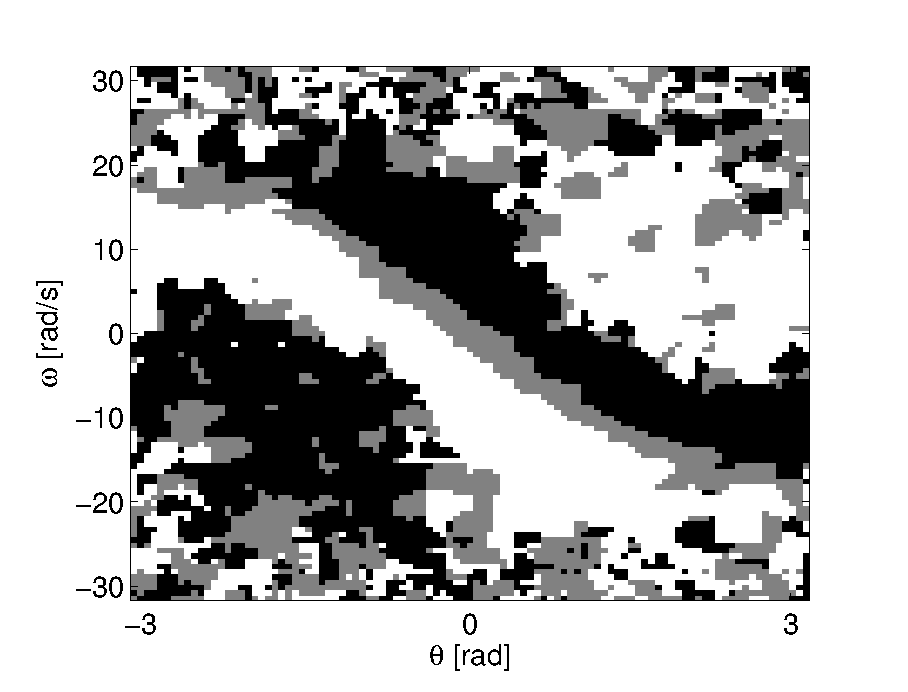
\includegraphics[width=.4\textwidth]{Figures/PS-LA4_policy}
\label{fig:PS-LA4_policy}
} 
\caption[Final policy using \acs{LA Dyna}]{Comparison of the final policies using \ac{LA Dyna}. \subref{fig:PS-LA1_policy}, \subref{fig:PS-LA2_policy}, \subref{fig:PS-LA3_policy} and \subref{fig:PS-LA4_policy} show the obtained policies using \acs{LLR} with increasing prediction interval limits. The white, gray and black areas correspond to control voltages of +3V, 0 and -3V respectively.}
\label{fig:PS-LA_policies}
\end{figure}


